\documentclass[hebrew, a4paper]{article}

\usepackage{amsmath, amssymb, amsfonts, amsopn, amsthm}
\usepackage{fancyhdr}
\usepackage{graphicx}
\usepackage{tikz, pgfplots}
\usepackage{xcolor}
\usepackage{mathtools, unicode-math, lualatex-math}
\usepackage{siunitx}

\usepackage{minted}
\setminted{fontsize=\footnotesize, stripnl}
\usepackage[hebrew, bidi=basic, layout=lists footnotes captions
extras sectioning tabular, provide={onchar=ids fonts, alph=letters.plain, Alph=letters}]{babel}
\usepackage{csquotes}
\usepackage[margin=2.5cm]{geometry}
\usepackage[skip=0.5em]{parskip}
\usepackage[hidelinks]{hyperref}

\linespread{1.15}

\babelprovide[onchar=fonts letters]{english}

\directlua {
  local function font_found(name)
  local foundname, subfont = luaotfload.aux.resolve_fontname(name)
  return (foundname and true) or false
  end

  local function make_fallback(names)
  local result = {}
  for _, name in ipairs(names) do
  if font_found(name) then
  table.insert(result, "name:" .. name .. ":mode=harf")
  end
  end
  return result
  end

  luaotfload.add_fallback("hebrewrm", make_fallback({
    "David CLM",
    "Hadasim CLM",
    "Liberation Serif",
    "FreeSerif"
  }))

  luaotfload.add_fallback("hebrewsf", make_fallback({
    "Nachlieli CLM",
    "Liberation Sans",
    "FreeSans"
  }))

  luaotfload.add_fallback("hebrewtt", make_fallback({
    "Liberation Mono",
    "FreeMono"
  }))
}

\babelfont{rm}[Ligatures=TeX]{TeX Gyre Pagella}
\babelfont{sf}[Ligatures=TeX]{TeX Gyre Heros}
\babelfont{tt}[Ligatures=TeX]{Liberation Mono}

\babelfont[hebrew]{rm}[RawFeature={fallback=hebrewrm}]{David CLM}
\babelfont[hebrew]{sf}[RawFeature={fallback=hebrewsf}]{Nachlieli CLM}
\babelfont[hebrew]{tt}[RawFeature={fallback=hebrewtt}]{Liberation Mono}

\babeltags{english=english}
\babeltags{hebrew=hebrew}

\setmathfont{Latin Modern Math}
\setmathfontface\mathrm{Latin Modern Math}

\pagestyle{fancy}
\fancyhf{}
\fancyhead[R]{\textsl{\leftmark}}
\fancyhead[L]{זיהוי קול}
\fancyfoot[C]{\thepage}

\usetikzlibrary{calc}
\pgfplotsset{compat=1.18}

\newcommand\downloadfile[2]{%
  \IfFileExists{#1}{}{\directlua{
      os.execute([[mkdir -p "`dirname #1`"]])
      os.execute([[curl -Lo #1 #2]])
  }}%
}

\renewcommand\cite[1]{}
\providecommand\parencite[1]{}
\providecommand\textcite[1]{}

\NewDocumentCommand\encite{m}{\textenglish{\cite{#1}}}
\NewDocumentCommand\enpcite{m}{\textenglish{\parencite{#1}}}
\NewDocumentCommand\entcite{m}{\textenglish{\textcite{#1}}}

\let\oldinputminted\inputminted
\RenewDocumentCommand\inputminted{o m m}{\begin{otherlanguage}{english}\oldinputminted[\IfNoValueF{#1}{#1}]{#2}{#3}\end{otherlanguage}}

%% Definitions
\theoremstyle{plain}
\newtheorem{theorem}{\theoremname}[section]

\theoremstyle{definition}
\newtheorem{definition}{\definitionname}[section]

\numberwithin{equation}{section}

%% Math commands
\DeclarePairedDelimiter\abs{\lvert}{\rvert}
\DeclarePairedDelimiter\norm{\lVert}{\rVert}
\DeclarePairedDelimiter\set{\{}{\}}
\DeclarePairedDelimiter\floor{\lfloor}{\rfloor}
\DeclarePairedDelimiter\ceil{\lceil}{\rceil}

\DeclareMathOperator\FAR{FAR}
\DeclareMathOperator\FRR{FRR}
\DeclareMathOperator\TAR{TAR}
\DeclareMathOperator\TRR{TRR}

\DeclareMathOperator*\argmax{arg\,max}
\DeclareMathOperator*\argmin{arg\,min}

\newcommand\andautoref[3]{%
  \setlocalecaption{#1}{#2}{#3}%
  \setlocalecaption{#1}{#2autoref}{#3}%
}

\setlocalecaption{hebrew}{figureautoref}{איור}
\setlocalecaption{hebrew}{tableautoref}{טבלה}
\setlocalecaption{hebrew}{sectionautoref}{פרק}
\setlocalecaption{hebrew}{subsectionautoref}{תת־פרק}
\setlocalecaption{hebrew}{subsubsectionautoref}{סעיף}
\setlocalecaption{hebrew}{appendixautoref}{נספח}

\andautoref{hebrew}{theorem}{משפט}
\andautoref{hebrew}{definition}{הגדרה}
\andautoref{hebrew}{equation}{משוואה}
\andautoref{hebrew}{listing}{קטע~קוד}

\andautoref{english}{theorem}{Theorem}
\andautoref{english}{definition}{Definition}
\andautoref{english}{listing}{Listing}

\setlocalecaption{hebrew}{listlisting}{רשימת קטעי הקוד}

\renewcommand\listingscaption{\listingname}
\renewcommand\listoflistingscaption{\listlistingname}

%% Colours
\definecolor{schoolgreen}{RGB}{47, 79, 79}

%% Resources
\downloadfile{images/school-logo.jpg}{https://dalet.school/wp-content/uploads/2024/08/Untitled-design-8.jpg}

%% ToC
\setcounter{tocdepth}{2}

\begin{document}
\begin{titlepage}
  \begin{center}
    \includegraphics[width=0.4\textwidth]{images/school-logo.jpg}
    \vspace{2cm}
    
    {\Huge\bfseries פרויקט גמר}
    \vspace{1cm}
    
    {\LARGE\bfseries בנושא}
    \vspace{0.5cm}
    
    {\LARGE\bfseries \textcolor{schoolgreen}{זיהוי קול}}
    \vspace{2cm}
    
    {\Large
      במסגרת~לימודי הנדסת תוכנה\\
      התמחות למידת מכונה ולמידה עמוקה\\
      5~יחידות לימוד
    }
    \vspace{2cm}

    \begin{Large}
      \begin{tabular}{r@{\hspace{2cm}}l}
        \textbf{מגיש:} & יונתן דפנא \\[0.3cm]
        \textbf{ת״ז:} & 333017192 \\[0.3cm]
        \textbf{מנחה:} & ד״ר שי פרח
      \end{tabular}
    \end{Large}

    \vfill
    {\Large\bfseries יוני 2026}
  \end{center}
\end{titlepage}

\tableofcontents
\newpage

\section{מבוא ותקציר}
\label{sec:introduction}

רבים המקרים בחיינו הדיגיטלים בהם צריך לאמת את~זהותו של~אדם מסוים,
ובהתאמה רבות המערכות המבקשות לסייע בנושא: הזדהות באמצעות סיסמה, טביעות
אצבע, סריקת פנים, ועוד. אבל שיטה לא כל כך נפוצה לזהות אנשים היא
באמצעות \emph{קולם}.

לפרויקט~הזה מטרה פשוטה מאוד; לשמש בסיס למערכת שיכולה לזהות אנשים
באמצעות ”טביעת הקול” שלהם. ברמה המעשית, הפרויקט נותן כלי שיכול להשוות
בין~שתי הקלטות שונות ולנחש, ניחוש מושכל של מודל קונבולוציה, האם~מדובר
באותו דובר.

בפרויקט~הזה לא ממומש רק מודל~אחד, אלא ארבעה (בשלוש~ארכיטקטורות שונות).
אבל כולם הם~מודלי קונבולוציה, שכן הקלטת קול, כמו תמונה, היא~בעלת מבנה
מרחבי וקונבולוציה היא~כלי מצוין לשמור על~המבנה המרחבי של~הקלט. אחת
ממטרות הפרויקט היא להשוות בין הארכיטקטורות השונות ולראות איזו מהן הכי
מתאימה למשימה.

כל המודלים אומנו באותה גישה, של למידה ניגודית (contrastive learning)
באמצעות triplet loss. זו השיטה שעבדה הכי טוב בניסיונות, ומגיעה להישגים
של כ-$\SI{85}{\percent}$ דיוק על מערך הנתונים המוגבל שהמודלים אומנו
עליו (ראו \autoref{sec:dataset}).

ניתן לראות הדגמה בקישור: \url{https://example.com}.

\subsection{פתרונות קיימים}
\label{sec:prior-art}

מודלים לסיווג (זיהוי דובר) ומודלים נידוגיים (אימות דובר) בדרך כלל לא
שונים ברמת המבנה, אלא רק בשכבות החיצוניות שלהם: מודלי סיווג פולטים
קטגוריה, ומודלי אימות עוצרים בשלב ה-embedding.

אחד מהמודלים הקיימים למשימה כזאת הוא VGGVox (\enpcite{voxceleb2})
שמבוסס על מערך הנתונים VoxCeleb2. הפרויקט~הזה לא שונה בתכלית מ-VGGVox,
אבל שונה בפרטי המימוש והארכיטקטורה: VGGVox אומנה מראש לסיווג ולאחר מכן
בעזרת contrastive loss, בעוד שכל המודלים בפרויקט הזה אומנו אך ורק עם
triplet loss. בנוסף, VGGVox פועלת על ספקטרוגרמה לינארית, בעוד שהמודלים
בפרויקט הזה שפועלים על ספקטרוגרמה, פועלים על ספקטרוגרמת לוג-Mel (ראו
\autoref{sec:mel-spectrogram}).

\subsection{המודלים}
\label{sec:intro-models}

הפרויקט כולל שלושה ”רעיונות” כלליים למודלים, שממומשים בארבעה~מודלים
שונים. כולם הם~מודלי קונבולוציה עם~שאריות (\enpcite{resnet}) שמאומנים
בטכניקות של contrastive learning, וניתן לקרוא עליהם עוד
ב\autoref{sec:architecture}.
\begin{enumerate}
\item רשת קונבולוציה חד-ממדית שעובדת על נתוני האודיו הגולמי, כלומר על
  מערך של~דגימות (samples) --- מודל אחד.
\item רשת קונבולוציה חד-ממדית שעובדת על ספקטרוגרמה, כלומר, ציר הזמן
  נשמר וכל קבוצה של תדרים קרובים (תא של תדרים) הוא feature התחלתי ---
  מודל אחד.
\item רשת קונבולוציה דו-ממדית שעובדת על ספקטרוגרמה, כלומר, מתייחסת
  לגרף העוצמה-תדר-זמן כתמונה דו-ממדית~--- שני מודלים;
  \begin{itemize}
  \item מודל אחד שמשתמש בארכיטקטורת MobileNetV2
    (\enpcite{mobilenetv2}), לא מאומנת מראש, לצד preprocessing.
  \item מודל אחד שמגדיר רשת קונבולוציה דו-מדדית סטנדרטית עם~שאריות.
  \end{itemize}
\end{enumerate}

\subsection{תוצאות עיקריות}
\label{sec:intro-results}

כל המודלים הגיעו ל-EER (\autoref{defn:eer}) בין $\SI{12.8}{\percent}$
ל-$\SI{18.9}{\percent}$, שמתאים לדיוק בין $\SI{81.1}{\percent}$
ל-$\SI{87.2}{\percent}$ על ה-dev set (ראו \autoref{sec:dataset}
לחלוקה). המספרים האלה לא מדהימים, וב\autoref{sec:discussion} מועלות
סיבות אפשריות. בנוסף, מדדי ה-AUC (\autoref{defn:auc}) נעים בין
$\num{0.89}$ ל-$\num{0.94}$.

\section{הגדרת הבעיה כבעית למידת מכונה}
\label{sec:problem-as-ml}

כל מודל בפרויקט הוא בסופו של דבר מודל embedding, כלומר, הפלט שלו לא
מועיל ישירות למשתמש ונועד לעיבוד נוסף על־ידי~האפליקציה. הקלט הוא קטע
שמע בעל ערוץ אחד (מונו) באורך שתי~שניות ובתדר דגימה (sample~rate)
של~$\num{16000}$ דגימות בשניה (ניתן לשנות בקלות את~שני הפרמטרים בקוד).
השמע מתקבל בפורמט גולמי --- כטנזור של דגימות (samples) בעל ממדים
\[
  \symit{shape}_x = (\num{32000}, 1)
\]
כי $\SI{2}{\s} \times \SI{16000}{\Hz} = \num{32000}$.

המשימה העיקרית של~המודל היא לבצע embedding, כלומר, לפלוט וקטור רב-ממדי
כלשהו (במקרה הזה $\num{2048}$) ומנורמל-$L_2$, שאמור להכיל מספיק מידע
על הדובר כך שעל־ידי בחירה מושכלת של מרחק~סף (\verb|threshold| או
\verb|margin|) ניתן להחליט אם הקטעים הוקלטו על־ידי~אותו דובר, או לא.
כלומר ממדי הפלט הם~$\symit{shape}_y = (\num{2048})$, ונחליט ששני קטעים
($y_1,y_2$) הוקלטו על־ידי~אותו דובר אם
\[
  \norm{y_1 - y_2} < \symit{margin}.
\]
על־מנת~לאמן מודל לבצע משימה כזאת, קיימות שתי פונקציות הפסד נפוצות:
\hyperref[sec:contrastive-loss]{הפסד ניגודי} (contrastive loss)
ו\hyperref[sec:triplet-loss]{הפסד־שלישיות} (triplet loss). מביניהן,
הפסד־שלישיות הוא חדש יותר וגם פשוט יותר, ולכן הוא זה שמשמש בפרויקט.

קשה למדוד את הדיוק (accuracy) של מודל embedding ישירות, כי המדד תלוי
בבחירת מרחק הסף. על~כן פותחו מספר מדדים להתמודד עם הבעיה הזו:
\textenglish{\hyperref[defn:eer]{EER (Equal Error Rate)}}
ו-\textenglish{ROC Curve (Receiver Operating Characteristic)}. ראו
\autoref{sec:contrastive-learning} למידע נוסף על פונקצית~ההפסד
ומדדי~ההצלחה.

\section{רקע תאורטי}
\label{sec:theory}

\subsection{על רשתות נוירונים}
\label{sec:neural-networks}

פריצות דרך רבות מאוד בתחום מדעי המחשב ומדעים באופן כללי נתקבלו מחיקוי
של המנגנונים הביולוגים של החי, ורשתות נוירונים הן אחת מהן. המוח מורכב
ממספר~רב של~תאי~עצב (נוירונים), כשלכל אחד קלט (דנדריט) ופלט (אקסון),
ושניהם מחוברים למספר תאי~עצב אחרים. נוירון יכול לפעול או לא לפעול (אין
לו דרגות שונות של פעילות), והוא עושה זאת על־פי האותות שהוא מקבל
מהדנדריט שלו.

רשת הנוירונים בתחום הבינה המלאכותית היא יישום מופשט מעט של עקרונות
דומים. גם בה יש ”נוירון” שמקבל קלט מנוירונים אחרים ופולט לנוירונים
אחרים. בניגוד לנוירון ביולוגי, הנוירון הממוחשב אינו בינארי, ויכול
לפלוט כל מספר ממשי. לכל~חיבור בין נוירונים (ניתן לחשוב על~החיבורים
כקשתות בגרף מכוון) משויך גם מספר, שנקרא המשקל (weight) של החיבור.
בנוסף, לכל נוירון משויך פרמטר bias והוא מחשב את הקלט שלו על־ידי צירוף
לינארי של פלטי הנוירונים שאליהם הוא מחובר.

משפט מאוד בסיסי ויסודי באלגברה הוא שהרכבה של~העתקות לינאריות היא בעצמה
העתקה לינאריות (וזה כולל גם העתקות עם איבר bias), ולכן אם היה הנוירון
פולט את הקלט שלו ישירות, כל הרשת למעשה הייתה מהווה העתקה לינארית אחת,
שאין בה כוח רב לפתרון בעיות.

\subsubsection{פונקצית אקטיבציה}
\label{sec:activation}

לנוירונים ביולוגיים יש ערך סף שבו הם מתחילים לפעול. עקרונית, היה אפשר
לממש מנגנון כזה גם במחשב בעזרת פונקצית מדרגות (step function), אבל
פונקציה כזאת אינה רציפה (ובוודאי אינה גזירה), מה~ששולל כל יכולת
אופטימיזציה (ראו \autoref{sec:optimization}). לכן הצירוף הלינארי של
קלטי הנוירון עובר דרך פונקצית אקטיבציה (activation function) \emph{לא
  לינארית} וגזירה.

\paragraph{טנגנס היפרבולי ($\tanh$)}

זוהי אחת מפונקציות האקטיבציה המוקדמות ביותר. מאפייניה העיקריים הם
שערכה חסום בתחום $(-1,1)$, והיא פונקציה אי-זוגית, כלומר, סימטרית ביחס
לאפס.

\paragraph{סיגמויד}

פונקצית הסיגמויד, או הפונקציה הלוגיסטית, דומה בצורתה ל-$\tanh$ אבל
פולטת ערכים בקטע $(0,1)$, ולכן היא שימושית כשנדרש פלט שמקרב הסתברות.
גם לסיגמויד וגם ל-$\tanh$ מאפיין בעייתי משותף, והוא שנגזרתם שואפת לאפס
ככל שערך הקלט גדל. זה דבר שיכול להקשות על אופטימיזציה
(\autoref{sec:optimization}).

\paragraph{ReLU}

זו אחת מפונקציות האקטיבציה השכיחות ביותר כיום, והיא זו שמשמשת בפרויקט
הנוכחי. הגדרתה פשוטה:
\[
  \mathrm{ReLU}(x) =
  \begin{cases}
    0 & x \leq 0 \\
    x & x \geq 0
  \end{cases}
\]
אבל היא עוצמתית מספיק כדי להתמודד עם משימות מורכבות.

\subsubsection{המבנה השכבתי של רשתות נוירונים}
\label{sec:layers}

אף שעקרונית ניתן לממש כל מבנה של גרף מכוון חסר~מעגלים כרשת נוירונים,
רוב היישומים כיום מחלקים את הנוירונים לשכבות, כשלכל נוירון מותר לקבל
קלט רק מהשכבה הקודמת ולפלוט פלט רק לשכבה הבאה (השכבה ה”אפס” היא הקלט
של כל הרשת).

בדרך כלל, לכל הנוירונים בשכבה אותה פונקצית אקטיבציה, ולכן ניתן להתייחס
לשכבה כולה כוקטור יחיד. מאחר שמטריצות מקודדות העתקות לינאריות, מעבר
משכבה אחת לבאה הוא למעשה כפל של השכבה הקודמת במטריצה, הוספת ה-bias,
והחלת האקטיבציה איבר-איבר.
\[
  \vec{a}_{n} = s(W_n\vec{a}_{n-1} + \vec{b}_n)
\]
פעולות לינאריות על וקטורים הן משהו שמחשבים, ובעיקר כרטיסי גרפיקה (GPU)
יודעים לעשות טוב מאוד, וזה מבטיח תהליכי חישוב יחסית מהירים.

התהליך הזה --- של כפל במטריצה, הוספת ה-bias, ואקטיבציה, לאורך כל שכבות
הרשת, נקרא forward pass וכך מחושב הפלט הסופי של המודל.

\subsection{אופטימיזציה}
\label{sec:optimization}

כשרוצים להגדיר מטרה חישובית בצורה מתמטית הרבה פעמים כדאי למצוא מספרים
שמתארים אותה. הרעיון מאחורי תהליך הלמידה העמוקה הוא פשוט: למצוא
פונקציה חיובית שמתארת את הביצועים של הרשת כתלות בפרמטרים (הם המשקלים
של שכבות הנוירונים), כלומר ”כמה היא גרועה”, ולהשתמש בטכניקות מהחשבון
הדיפרנציאלי על־מנת~למזער אותה.

\subsubsection{פונקצית עלות ופונקצית הפסד}
\label{sec:cost-and-loss}

הנתונים שאותם מלמדים את הרשת מורכבים בדרך כלל מרשימה של דוגמאות. לכל
דוגמה, ניתן למדוד כמה הרשת מזייפת בחישוב התשובה של הדוגמה המסוימת
הזאת; זה ה”הפסד” (loss). לאחר מכן סוכמים את ההפסדים על כל הדוגמאות
ומקבלים את ה”עלות” (cost) של~הרשת על~כל~מערך הנתונים.

מפונקצית עלות נדרש בדרך כלל ש”תתנהג יפה”, כלומר, תהיה גזירה ולא תגזים
או תמעיט בערך טעות הרשת.

\subsubsection{Back-propagation}
\label{sec:backpropagation}

מאחר שדאגנו שפונקציות האקטיבציה ופונקצית ההפסד יהיו גזירות, כל פעולת
הרשת, מקלט ועד עלות, היא פונקציה גזירה שתלויה בכל הפרמטרים:
\[
  J(W_1,b_1,\ldots,W_n,b_n),
\]
כש-$W$ היא משפחה של~מטריצות משקלים ו-$b$ היא משפחה של~וקטורי bias.

הצעד הראשון הדרוש בשביל למזער פונקציה הוא לגזור אותה, ועבור פונקציה
מרובת משתנים כזאת, מדובר בלמצוא את כל הנגזרות החלקיות שלה (הגרדיאנט).
אם אנחנו יודעים לגזור את פונקצית האקטיבציה ופונקצית העלות (כפונקציה של
הפלט), ניתן להשתמש בכלל השרשרת על־מנת למצוא את הנגזרות החלקיות של
פונקצית העלות (כפונקציה של המשקלים). קיימות מספר טכניקות לגזירה.

\paragraph{גזירה נומרית}

גזירה נומרית היא קירוב הנגזרת על־ידי הגדרתה:
\[
  \frac{\partial \vec{f}}{\partial x}(x_0,\ldots) = \lim_{h \to 0} \frac{\vec{f}(x_0+h,\ldots) - \vec{f}(x_0,\ldots)}{h}
\]
כלומר, חישוב הביטוי בתוך הגבול לערכים קטנים של $h$ והכפלת הנגזרות
החלקיות אחת בשנייה לפי~כלל השרשרת. החישוב יחסית פשוט, אבל קשה לדעת
אילו ערכים של $h$ הם קטנים מספיק וכך מאבדים דיוק. בנוסף, צריך לבצע
חישוב נפרד לכל משתנה קלט.

\paragraph{גזירה סימבולית}

מכיוון שכל הפונקציות שאנחנו עובדים איתן הן פונקציות שקבענו מראש, אנחנו
כבר יודעים איך לגזור אותן. גזירה סימבולית מנתחת את קוד המקור של הרשת
ומייצרת פונקצית נגזרת באופן מפורש על־פי~כללי גזירה ידועים. הנגזרת תהיה
תמיד מאוד מדויקת, אבל החישוב הוא מסובך, דורש זיכרון רב ודרוש לנתח קוד
מקור.

\paragraph{גזירה אוטומטית}

גזירה אוטומטית דומה לגזירה סימבולית בכך שהיא משתמשת בנגזרות של
פונקציות ידועות ובכללי גזירה ידועים על־מנת~לחשב נגזרות של פונקציות
מורכבות, אבל היא מתבצעת בשיטה אחרת לגמרי (\enpcite{autodiff}).

\subparagraph{גזירה אוטומטית קדמית}

גזירה אוטומטית קדמית מתבצעת לכל משתנה קלט בנפרד. כל ערך מספרי בפונקציה
סוחב איתו גם את~נגזרתו הראשונה, ובכל קריאה לפונקציה, מחושבת הנגזרת
החלקית על־פי כללי גזירה ידועים, עד שמגיעים לעלות. כך החישוב מתבצע
”מבפנים החוצה”.

\subparagraph{גזירה אוטומטית אחורית}

גזירה אוטומטית אחורית מתבצעת לכל משתנה פלט בנפרד, ולכל משתני הקלט
ביחד. התהליך מתחיל בחישוב רגיל של הפונקציה, המכונה forward pass, ובו
נבנה גם גרף חישוב המתחזק את קשרי התלות בין ערכים מספריים שונים. השלב
השני, המכונה backwards pass, מתבצע מאחד מהעלים של הדרף (משתנה פלט)
אחורה ומחשב את~הנגזרות החלקיות המתאימות לכל קשת, עד שבסוף מגיעים לכל
משתני הקלט.

מאחר שברצוננו לחשב את הנגזרת של העלות, שהוא מספר יחיד, ברור שעדיף
להשתמש בגזירה אוטומטית אחורית, שכן גזירה אוטומטית קדמית מתבצעת לכל
משתנה קלט בנפרד!

בתחום הלמידה העמוקה, תהליך ה\emph{גזירה האוטומטית האחורית} נקרא גם
Back-propagation, וזו הדרך המקובלת לחשב את גרדיאנט העלות.

\subsubsection{Gradient Descent}
\label{sec:gradient-descent}

עבור פונקציה מרובת-משתנים גזירה (יש לשים לב שקיום הנגזרות החלקיות לא
מבטיח גזירות), המכפלה הסקלרית של הגרדיאנט בוקטור יחידה כלשהו היא
הנגזרת הכיוונית של הפונקציה לאורך אותו הוקטור. בפרט, מאי-שוויון קושי-שוורץ
\[
  \abs{\vec{u} \cdot \vec{v}} \leq \norm{\vec{u}}\norm{\vec{v}}
\]
נובע שהנגזרות הכיווניות הכי גדולות, בערך מוחלט, הן בכיוון הגרדיאנט
עצמו ובכיוון המנוגד לו בדיוק. מכאן שהירידה הכי תלולה בגרף הפונקציה
תימצא בכיוון המנוגד לגרדיאנט (מכפלה סקלרית של שני וקטורים המצביעים
באותו כיוון היא תמיד אי-שלילית, ושל וקטורים המצביעים בכיוונים מנוגדים
תמיד אי-חיובית).

אלגוריתם האופטימיזציה הכי פשוט, המכונה gradient descent, מחסיר בכל צעד
מהמשקלים הנוכחיים את הגרדיאנט, מוכפל בערך קטן $\alpha$, המכונה
\emph{שיעור הלמידה} (ה-learning rate).
\[
  \vec{\theta}_{n+1} = \vec{\theta}_{n} - \alpha \nabla J(\vec{\theta}_n)
\]
כש-$\vec{\theta}$ מתייחס לוקטור של כל~המשקלים ביחד, והמשקלים מאותחלים
ל-$\vec{\theta}_0$ באופן אקראי.

הבעייה העיקרית ב-gradient descent היא שלא תמיד אפשרי לחשב את הגרדיאנט
עבור כל הנתונים ביחד, מפאת מגבלות זיכרון, ולכן מקובל לעבוד במקבצים
(batches) --- זה נקרא stochastic gradient descent. ומאחר שמקבץ לא מתאר
במדויק את כל הנתונים, ביצוע gradient descent למקבצים שונים נדמה למסלול
הליכתו של אדם שיכור (במרחב הרב-ממדי של~משקלי הרשת).

\subsubsection{Adam}
\label{sec:optimization-adam}

מספר אלגוריתמים פותחו להתמודד עם~החסרונות של gradient descent.

\paragraph{Adagrad}

האלגוריתם הזה (\enpcite{adagrad}) מבוסס על רעיון יסודי אחד: שיעור
הלמידה לא זהה לכל הפרמטרים, אלא הוא וקטור, כלומר, שיעור למידה נפרד לכל
פרמטר. שיעור הלמידה הזה מחושב בפרופורציה לשורש ההופכי של סכום ריבועי
הנגזרות החלקיות עד כה, כך שהוא קטן עם הזמן וככל שהנגזרות גדלות, מה
שתורם להתכנסות. המטרה העיקרית של האלגוריתם היא למנוע את ה”זיגזג” שנוצר
בעקבות stochastic gradient descent.

\paragraph{RMSProp}

האלגוריתם הזה מאוד דומה ל-Adagrad ונועד לשפר את ביצועיו. במקום לשמור
סכום של \emph{כל} הגרדיאנטים הקודמים, RMS\-Prop שומר ממוצע נע (ממוצע על
חלון) של~גרדיאנטים קודמים וכך תהליך האופטימיזציה לא נתקע.

\paragraph{Adam}

זה אלגוריתם האופטימיזציה שמשמש בפרויקט~הזה (\enpcite{adam}). הוא מבוסס
על RMSProp. במקום ממוצע של ריבועי הגרדיאנטים, Adam מתחזק שני ממוצעים
נעים מעריכיים: של הגרדיאנט עצמו (מקרב את הממוצע) ושל ריבועו (מקרב את
השונות, או~variance). שני היפר-פרמטרים מבקרים את~שיעור הדעיכה של
הממוצעים~האלה.

גודל הצעד של Adam פרופורציונלי לממוצע הראשון, והופכי לשורש הממוצע
השני. כך ה\emph{כיוון} הכללי של הגרדיאנט נשמר, אבל תנועת הלוך-חזור
בזיגזג מצומצמת.

\subsection{בעיות ה-Overfitting ו-Underfitting}
\label{sec:overfitting-underfitting}

אם מבנה הרשת לא מספיק טוב, או אלגוריתם האופטימיזציה מתקשה, או שאין
מספיק נתונים, הרשת לא תלמד כראוי וביצועיה לא יהיו טובים על שום קלט.
מצב כזה נקרא תת-התאמה (Underfitting).

מצד שני, אם מבנה הרשת עמוק או מסובך מדי, או שאין מספיק נתונים, יכול
להיות שהרשת ”תלמד בעל־פה” את נתוני האימון שלה, במקום להכליל תבניות.
הרשת תראה ביצועים טובים מאוד על נתוני האימון אבל פחות טובים על נתונים
שהיא לא ראתה מעולם. מצב כזה נקרא התאמת־יתר (Overfitting).

יש לציין שדרך מצוינת להתמודד גם עם Overfitting וגם עם Underfitting היא
\emph{יותר נתונים}. חוץ מזה, לכל בעיה יש דרכים משלה.

\subsubsection{דרכים להתמודד עם Underfitting}
\label{sec:underfitting-solutions}

בנוסף לחוסר בנתונים, Underfitting הרבה פעמים נגרם כי הרשת לא מספיק
טובה לקודד את~הבעיה. בדרך כלל ניתן לפתור את זה על־ידי הוספת שכבות
נוספות והגדלת שכבות קיימות, בשביל להגדיל את יכולת העיבוד של הרשת.

חוץ מזה, לפעמים ניתן לעבד את הנתונים מראש (לבצע preprocessing, ראו גם
\autoref{sec:dataset}) על־מנת להביא אותם לצורה שהרשת תוכל ללמוד יותר
טוב. רשתות נוירונים בדרך כלל אוהבות מספרים בין $-1$ ל-$1$, למשל.

\subsubsection{דרכים להתמודד עם Overfitting}
\label{sec:overfitting-solutions}

בנוסף לחוסר בנתונים, Overfitting הרבה פעמים נגרים ממבנה רשת מסובך מדי.
ניתן לפעמים לפשט את מבנה הרשת: למחוק או להקטין שכבות. בנוסף, קיימות
מספר טכניקות רגולריזציה שכולן נועדו לשפר את ביצועי הרשת על~נתונים שהיא
מעולם לא ראתה.

\paragraph{Dropout}

הרעיון מאחורי השיטה הזאת הוא שאנחנו לא רוצים שהרשת תסתמך יותר מדי
על~נוירונים מסוימים (שעלולים ”ללמוד בעל פה” נתונים), אלא על~המבנה
הכללי שלה. טכניקת ה-Dropout חלה על שכבה מסוימת או מספר שכבות, ובמהלך
הלמידה היא מכבה, כלומר משביתה, חלק מהנוירונים בשכבה (מקובל להשבית
$\SI{20}{\percent}$). במהלך פעולה רגילה של הרשת (נקראת גם inference),
כל הנוירונים עובדים.

\paragraph{Early Stopping}

לפעמים Overfitting נגרם כי מאמנים את הרשת יותר מדי. עצירה מוקדמת
(Early Stopping) מפסיקה לאמן את הרשת כשביצועיה על~נתונים שלא אומנה
עליהם מפסיקים להשתפר, בדרך כלל עם קצת סבלנות לשיפורים מאוחרים.

\paragraph{Batch Normalization}

כפי שמרמז השם, זו פעולה שחלה על כל מקבץ (batch) בנפרד. למעשה אלה שכבות
ברשת, ובמהלך האימון הן מזיזות ומותחות את הקלט על־מנת~להזיז את הממוצע
ל-$0$ ואת סטיית התקן ל-$1$. במהלך inference, אין טעם להסתמך על הקלט
באופן ישיר, ובמקום זאת שכבות ה-Batch Normalization מבצעות נורמליזציה
קבועה לפי~המאפיינים של נתוני האימון.

\paragraph{רגולריזצית $L_2$}

הרעיון מאחורי רגולריזצית-$L_2$ הוא להעניש את הרשת על משקלים גדולים.
היא מתבצעת על־ידי הוספת גדלי המשקלים לפונקצית העלות.

הפרויקט~הזה לא משתמש ברגולריזצית-$L_2$.

\paragraph{אוגמנטציה}

אוגמנטצית נתונים (data augmentation) מייצרת עוד דוגמאות נתונים באופן
מלאכותי. הנתונים החדשים מיוצרים אך ורק לפי הנתונים הקודמים, אבל עדיין
מספקים גיוון שעשוי למנוע Overfitting. על נתוני תמונה (דו-ממדית), אפשר
למשל לשקף, להגדיל, להקטין ולסובב תמונות, ונתוני שמע אפשר לחתוך בצורה
אקראית מספר פעמים שונות (ראו גם \autoref{sec:dataset-in-memory}).

\subsection{למידת ניגודים}
\label{sec:contrastive-learning}

ברשתות המבצעות סיווג (classification) מקובל בדרך כלל לסיים את הרשת
בכמה שכבות fully connected --- שכל נוירון בשכבה מחובר לכל נוירון בשכבה
הבאה --- כשהפלט הסופי הוא וקטור באורך מספר הקטגוריות, שרכיביו מקרבים
הסתברויות (פונקצית האקטיבציה של השכבה האחרונה תהיה בדרך כלל
הלוגיסטית).

רשתות שמטרתן לבצע embedding, כלומר, להעתיק את הקלט לוקטור רב-ממדי
כלשהו, לא דורשות את השכבה הסופית הזאת. למידת ניגודים היא אוסף של
טכניקות לאימון רשתות embedding. מערך הנתונים נותן תווית (label) לכל
דוגמה, והמטרה של הרשת היא להעתיק דוגמאות בעלות תווית זהה לוקטורים
קרובים, ודוגמאות בעלות תווית שונה לוקטורים רחוקים. נהוג לנרמל את כל
הוקטורים, כלומר לוודא שאורכם $1$.

\subsubsection{הפסד ניגודי ורשתות סיאמיות}
\label{sec:contrastive-loss}

מערך הנתונים מחולק לזוגות חיוביים (דוגמאות עם אותה תווית) וזוגות
שליליים (דוגמאות עם תוויות שונות). כדאי לכוון לכמות שווה בערך של זוגות
חיוביים ושליליים. אם $n$ הוא מספר הדוגמאות לתווית מסוימת, אז מספר
הזוגות החיוביים שניתן ליצור מהן הוא $\binom{n}{2}$.

לכל זוג ניתנת תווית ($y$) מספרית חדשה: $1$ לזוגות חיוביים ו-$0$ לזוגות
שליליים. פונקציות ההפסד מוגדרת עבור זוג וקטורי embedding מסוים $(a,b)$
על־ידי:
\begin{equation}
  \label{eq:contrastive-loss}
  \symcal{L}(a,b,y) = y\norm{a - b}^2 + (1-y)\max\set{(m - \norm{a-b})^2, 0}
\end{equation}
כש-$m$ הוא היפר-פרמטר. ניתן לראות שאם התווית היא $1$, כלומר הזוג
חיובי, הביטוי שקול ל-$\norm{a-b}^2$, ובשביל למזער אותו יש לקרב את
הוקטורים, ואם התווית היא $0$, כלומר הזוג שלילי, אז הביטוי הוא
$\max\set{(m-\norm{a-b})^2,0}$, ובשביל למזער אותו יש להרחיק את הזוג עד
מרחק $m$ לפחות.

רשת שמאומנת בהפסד ניגודי צריכה לקבל זוגות של קלטים ולהעתיק אותם לזוגות
של וקטורי embedding. השיטה המקובלת היא לבנות רשת שמטפלת בקלט אחד,
ולהצמיד שני עותקים שלה אחד לשני (מכאן הכינוי ”רשת סיאמית”). יש לציין
ששני העותקים חולקים פרמטרים, ומתאמנים תמיד ביחד. כך אפשר להגדיר
את~ההפסד הניגודי ולאמן את הרשת.

\subsubsection{הפסד שלישיות ורשתות משולשות}
\label{sec:triplet-loss}

מערך הנתונים מחולק הפעם לשלישיות, ללא תווית, כשרכיב הראשון בשלישייה
נקרא anchor, השני positive, והשלישי negative. המטרה היא לקרב את
ה-anchor ל-positive ולהרחיק ממנו את ה-negative.

\begin{listing}
  \inputminted{python}{snippets/TripletLoss.py}
  \caption{הפסד שלישיות (\autoref{eq:triplet-loss}). חלק מהפונקציות הושמטו.}
  \label{lst:triplet-loss}
\end{listing}

פונקצית ההפסד מוגדרת עבור שלישיית וקטורי embedding מסוימת $(a,p,n)$
על־ידי:
\begin{equation}
  \label{eq:triplet-loss}
  \symcal{L}(a,p,n) = \max\set{\norm{a-p}^2 - \norm{a-n}^2 + m, 0}
\end{equation}
כש-$m$ הוא היפר-פרמטר. ניתן לראות שעל־מנת למזער את פונקצית העלות, יש
לקרב את $a$ ל-$p$ ולהרחיק את $a$ מ-$n$ (עד הפרש של $m$ בין המרחקים).
בדרך כלל בוחרים את $m$ בטווח $[0.2,1]$.

כמו שהפסד~ניגודי דורש רשת סיאמית, הפסד~שלישיות דורש רשת משולשת. העקרון
זהה; בונים שלושה עותקים של אותה הרשת שחולקים פרמטרים ומאמנים אותם
ביחד. חישוב הפסד~שלישיות פשוט יותר וקל יותר לגזירה מהפסד~ניגודי, והוא
מגיע בדרך כלל לתוצאות טובות יותר. לכן כל המודלים בפרויקט הזה משתמשים
בהפסד שלישיות.

\subsubsection{מדדי הצלחה}
\label{sec:contrastive-metrics}

ברשת embedding, בדרך כלל מחליטים ששני קלטים מתאימים אם המרחק האוקלידי
בין וקטורי הפלט שלהם קטן מערך~סף מסוים. אי~אפשר למדוד את דיוק הרשת
ישירות, כי הדיוק תלוי בבחירת ערך~הסף (נסמן אותו $t$).

קודם כל, הנתונים מחולקים לזוגות כמו בהפסד~ניגודי. נסמן ב-$P$ את קבוצת
הזוגות החיוביים $\set{i \mid y^{(i)} = 1}$ וב-$N$ את קבוצת הזוגות
השליליים $\set{i \mid y^{(i)} = 0}$. נסמן ב-$\hat{y}$ את ה\emph{מרחק}
בין וקטורי ה-embedding של זוג מסוים.

נסמן ב-$A$ את קבוצת הזוגות שהרשת מקבלת כמתאימים:
$\set{i \mid \hat{y}^{(i)} < t}$ (אומרים שהרשת ”מקבלת” אותם) וב-$R$ את
קבוצת הזוגות שהרשת מקבלת כשונים: $\set{i \mid \hat{y}^{(i)} \geq t}$
(אומרים שהרשת ”דוחה” אותם). נציין ששתי הקבצות האלו תלויות בבחירה
של~$t$.

נציין גם שמאחר שהוקטורים מנורמלים, המרחק הכי גדול שיכול להיות בין
וקטורים הוא~$2$ (לפי אי-שוויון המשולש):
\[
  \norm{u - v} \leq \norm{u} + \norm{-v} = \norm{u} + \norm{v} = 2
\]
ולכן נגביל את $t$ לתחום $(0,2)$.

\begin{definition}[FRR]\label{defn:frr}
  שיעור הדחייה השגויה (False Rejection Rate) הוא שיעור הזוגות החיוביים
  שהרשת דחתה:
  \[
    \FRR(t) = \frac{\abs{P \cap R}}{\abs{P}}
  \]
\end{definition}

\begin{definition}[FAR]\label{defn:far}
  שיעור הקבלה השגויה (False Acceptance Rate) הוא שיעור הזוגות השליליים
  שהרשת קיבלה:
  \[
    \FAR(t) = \frac{\abs{N \cap A}}{\abs{N}}
  \]
\end{definition}

\begin{definition}[TAR]\label{defn:tar}
  שיעור הקבלה הנכונה (True Acceptance Rate) הוא שיעור הזוגות החיוביים שהרשת קיבלה:
  \[
    \TAR(t) = \frac{\abs{P \cap A}}{\abs{P}} = 1 - \FRR(t)
  \]
\end{definition}

ועכשיו אפשר להגדיר את המדד הראשון שלנו.

\begin{definition}[EER]\label{defn:eer}
  ערך~הסף האופטימלי הוא הערך בו ה-FAR וה-FRR שווים (או הכי קרובים):
  \[
    t_{\mathrm{optimal}} = \argmin_t \abs{\FAR(t) - \FRR(t)}
  \]
  ושיעור השגיאה השווה (Equal Error Rate) הוא אותו ערך ה-FAR וה-FRR:
  \[
    \operatorname{EER} \approx \FAR(t_{\mathrm{optimal}}) \approx \FRR(t_{\mathrm{optimal}})
  \]
\end{definition}

ערכי FAR ו-FRR, כפונקציות של $t$, אינן פונקציות רציפות, כי כמות
הנתונים היא סופית. אבל ניתן לקרב אותן טוב על־ידי פונקציות רציפות. FAR
היא פונקציה מונוטונית עולה, ו-FRR היא פונקציה מונוטונית יורדת לאותו
תחום ($[0,1]$), ושתיהן, כפונקציות רציפות, מכסות את כל התחום (הן
פונקציות על $[0,2] \to [0,1]$). לכן לפונקציות הרציפות שמקרבות את FAR
ו-FRR בטוח יש נקודת חיתוך, כלומר ה-EER קיים. ניתן לחשוב על ה-EER
כ”דיוק הטוב ביותר” של הרשת.

ראינו שה-FAR כפונקציה של $t$ עולה מונוטונית. גם ה-TAR עולה מונוטונית
כפונקציה של $t$, ולכן ניתן לצייר גרף של TAR מול FAR (במילים אחרות, גרף
של הנקודות $(\FAR(t),\TAR(t))$ לכל $t\in[0,2]$). מאחר שהפונקציות אינן
רציפות, הגרף לא יהיה בהכרח רציף, אבל הוא מגדיר בקירוב גרף של פונקציה
רציפה כמעט-בכל-מקום, כלומר אינטגרבילית. זה הוא גרף ה-ROC, או Receiver Operating Characteristic (ראו \autoref{fig:roc-example}).

\begin{figure}
  \centering
  \includegraphics[scale=0.4]{images/roc-example.png}\\
  הקו המקווקו מייצג את הישר $y=x$.
  \caption{דוגמה לגרף ROC}
  \label{fig:roc-example}
\end{figure}

\begin{definition}[AUC]\label{defn:auc}
  מדד השטח מתחת לגרף (Area Under the Curve) הוא השטח מתחת לגרף ה-ROC:
  \[
    \operatorname{AUC} = \int_0^1 \TAR~d\FAR
  \]
\end{definition}

ה-AUC כלוא תמיד בתחום בין $0$ ל-$1$ (כי השטח של הריבוע
$[0,1]\times[0,1]$ הוא $1$). ה-AUC הוא לא אותו דבר כמו דיוק, אבל עבור
רשת שמנחשת, נצפה שה-FAR וה-TAR יהיו שווים בערך, ואז נקבל AUC של $0.5$.
למעשה, ה-AUC הוא ההסתברות שהמרחק בין הרכיבים של זוג חיובי אקראי יהיה
קטן מהמרחק בין הרכיבים של זוג שלילי אקראי (\enpcite{roc}).

ניתן להעניק גם פרשנות גאומטרית למדד ה-EER; אם נצייר את הישר $y=1-x$ על
גבי \hyperref[fig:roc-example]{גרף ה-ROC}, שיעור ה-$x$ של הנקודה שבא
הוא חותך את הגרף הוא ה-EER.

\subsection{שכבות קונבולוציה}
\label{sec:convolution}

באופן מסורתי רשתות נוירונים השתמשו בשכבות fully connected, כלומר שכל
נוירון בשכבה מחובר לכל הנוירונים בשכבה הבאה. רשתות כאלה נקראות גם
Multi-layer Perceptron. אבל מתברר ששכבות FC כאלה לא כל כך מתאימות
לנתונים בעלי מבנה מרחבי מסובך. הן יכולות לעבוד לסיווג תמונות מאוד
קטנות למעט מאוד קטגוריות (כמו הפרצפטרון המקורי שעל שמו הן נקראות), אבל
לא הרבה יותר מזה.

במתמטיקה, הקונבולוציה היא פעולה יסודית בתורת ההסתברות. הגרסה הבדידה של
הקונבולוציה מצעידה ”חלון” של מספרים על גבי מערך יותר גדול של מספרים,
ומשתמשת במספרי החלון כמקדמים לחישוב צירופים לינאריים של איברי מערך
הקלט. הגרסה שמשתמשים בה בלמידה עמוקה מוסיפה גם bias.

קונבולוציה לא יכולה לעשות שום דבר ששכבת FC לא יכולה באופן תאורטי, אבל
הרבה יותר קל לאמן שכבות קונבולוציה מאחר שהן תמיד שומרות על המבנה
המרחבי של הקלט (\enpcite{cnn}).

במקום פרמטר לכל זוג נוירונים מתוך שכבות שכנות, לשכבת קונבולוציה יש
מספר פרמטרים קבוע, כגודל הפילטר (החלון הצועד) שלה, ועוד bias, כפול
מספר הערוצים בשכבה הקודמת, כפול מספר הפילטרים. פילטר אחד פועל על כל
ערוצי שכבת הקלט ביחד, עם פרמטרים נפרדים, ופולט שכבת קלט אחת.

עבור קונבולוציה חד-ממדית, אם $k$ הוא גודל הפילטר, $s$ הוא גודל הצעד
(stride) ו-$w$ הוא אורך הקלט, אז אורך הפלט יהיה
\[
  \floor*{\frac{w-k}{s}} + 1.
\]
מקובל לעתים להוסיף ריפוד (padding) על מנת שאורך הפלט יהיה זהה לאורך
הקלט.

נציין שמאחר שפעולת הקונבולוציה עדיין מורכבת מצירוף לינארי של רכיבי
הקלט, ניתן לקודד גם אותה כמטריצה (עם רכיבים רבים שחוזרים על עצמם)
ולנצל את יתרונות המהירות הטמונים בזה.

\subsection{שכבות שארית ו-Skip Connections}
\label{sec:skip-connections}

רשתות קונבולוציה עמוקות הרבה פעמים נתקלות בבעיות Overfitting
ו-Exploding gradients. הרעיון מאחורי skip connections הוא לאפשר לרשת
”לא לעשות שום דבר” באחת מהשכבות.

בשכבת קונבולוציה מסורתית, בשביל לקבל פרמטרים שלא משנים את הקלט, תהליך
הלמידה צריך לעבוד מאוד קשה; צריך למצוא בדיוק את הפרמטרים הנכונים בשביל
לעשות את זה. אם נתאר את הפלט של שכבה רגילה כ-$f(x)$, כש-$x$ הוא
האקטיבציות של השכבה הקודמת, אז שכבת שארית פולטת $x + f(x)$. בשביל
להשיג שכבה ש”לא עושה כלום” מספיק למצוא פרמטרים שגורמים לאקטיבציה $0$
(עבור פונקצית אקטיבצייה כמו ReLU זה קל, כי היא מתאימה כל מספר שלילי
ל-$0$). ראו את \autoref{sec:architecture} עבור המימוש של שכבות שארית
בפרויקט הזה.

\subsection{קלט שמע}
\label{sec:audio-input}

קטעי השמע מגיעים אלינו ממערך הנתונים (ראו \autoref{sec:dataset})
כקבצים במערכת (במקרה הזה FLAC), שצריך לקודד. כמו כן, יש לוודא שקצב
הדגימה (sample rate) זהה לכולם, ולכל קלט עתידי שהרשת תקבל, בשביל
להבטיח ביצועים אחידים. לאחר שדוגמים מחדש את הקבצים לקצב הנבחר, יש
לחתוך אותם לאורך אחיד.

מערך של דגימות הוא כבר מבנה שניתן לבצע עליו קונבולוציה חד-ממדית, וזה
באמת מה שאחד המודלים עושה (\autoref{sec:architecture-audiocnn}).

\subsubsection{ספקטרוגרמת Mel}
\label{sec:mel-spectrogram}

בני אדם לא חווים קול כדגימות יחידות, אלא כאוסף של גלים בתדרים שונים,
ומחקרים מסכימים ששם טמונים גם המאפיינים הייחודיים של כל קול. אפילו
ששכבת קונבולוציה יכולה, באופן תאורטי, לחלץ תדרים מתוך אות גולמי, מוטב
לעשות את זה בדרך יעילה ומהירה מראש, כך שהקונבולוציה ישר מידע על
התדרים.

\emph{התמרת פורייה} היא כלי מתמטי שממיר פונקציה מחזורית בסכום של גלי
סינוס. אנו מעוניינים בגרסה הבדידה שלה, שמכונה DFT, שתעבוד על קטעי קול
קצרים כל פעם, מה שמכונה Short-time Fourier Transform, או STFT. הפלט של
STFT הוא מבנה דו-ממדי הנקרא \emph{ספקטרוגרמה}. ספקטרוגרמה מייצגת תדרים
באופן לינארי, אבל בני אדם, והטבע, לא מתייחס לתדר באופן לינארי, אלא
באופן לוגריתמי.

סולם Mel (מ-Melody) הוא סולם תדרים שמייצג את ערכי התדרים באופן יותר
קרוב לדרך בה בני אדם באמת שומעים אותם. הנוסחה להמרה בין תדר
ביחידות~$\unit{\Hz}$ לסולם~Mel היא
\begin{equation}
  \label{eq:mel-scale}
  \operatorname{mel}(f) = \num{2595} \log_{10}\left(1 + \frac{f}{700}\right)
\end{equation}
והיא נקבעה ככה בשביל~ש-$\SI{1000}{\Hz} = \SI{1000}{Mel}$.

מתברר שאף יותר שימושי לעבוד עם הלוגריתם של ספקטרוגרמת~Mel, כי בני אדם
לא חווה רק תדר באופן לוגריתמי, אלא גם עוצמה. מאחר שהערכים המספריים של
הספקטרוגרמה הם עוצמות תדרים, שימוש בלוגריתם עוזר להבין עוצמה יחסית.
דוגמאות לספקטרוגרמות~לוג-Mel ניתן לראות
ב\autoref{sec:dataset-example-spectrograms}.

הספקטרוגרמה היא אובייקט דו-ממדי ולכן ניתן להריץ עליה קונבולוציה
דו-ממדית, או קונבולוציה חד-ממדית בממד הזמן. קונבולוציה דו-ממדית מאפשרת
להשתמש בטכניקות ידועות מעולם עיבוד התמונות, וקונבולוציה חד-ממדית
מאפשרת להתייחס לכל תחום התדרים ביחד.

\subsubsection{MFCC}
\label{sec:mfcc}

דרך אחרת לייצוג קלט שמע היא MFCC, שנגזרת מספקטרוגרמת Mel על־ידי פעולת
Direct cosine transform. הוא מייצג מאפיינים שונים של האות, שעשויים
להיות שימושיים למטרות זיהוי קול.

הפרויקט הזה לא משתמש ב-MFCC, כי רציתי לאמן מודלים על קלט דומה יחסית
למה שבני אדם מבינים. ספקטרוגרמה היא תצוגה יחסית אינטואיטיבית של קול,
ולכן זה התאים למשימה.

\subsubsection{בעיית ה-Aliasing}
\label{sec:frequency-limits}

אם באות מסוים קיימים רכיבים בתדר הגדול מחצי קצב הדגימה (תדר ניקוויסט
של הדוגם), הם יופיעו כתדרים נמוכים באות הדגום. משפט נייקוויסט-שאנון
מבטיח שדוגם בקצב מסוים יכול לייצג באופן מושלם פונקציות שאין להן רכיבים
בתדרים גבוהים.

\begin{theorem}[נייקוויסט-שאנון]\label{thm:nyquist-shannon}
  אם פונקציה $f(x)$ לא מכילה אות בתדר גדול מ-$B [\unit{\Hz}]$, אז ניתן
  לקבוע אותה לחלוטין על־ידי דגימתה בכל~קצב דגימה גדול מ-$2B$.
\end{theorem}

על־מנת להתמודד עם הבעייה הזו, נהוג להיפטר מכל התדרים הגבוהים לפני
הדגימה (בעזרת מסנן מעביר נמוכים), ובכל מקרה, תדרים כאלה (מעל חצי מקצב
הדגימה) לא יופיעו באות הדגום ולכן אין טעם להתייחס אליהם בספקטרוגרמה.

\section{כלים וסביבת פיתוח}
\label{sec:environment}

הפרויקט כתוב בפייתון~3.11, ומבוסס על Keras ו-PyTorch. רשימת ספריות
מלאה:
\begin{otherlanguage}{english}
\begin{verbatim}
numpy
matplotlib
importlib_resources
ipywidgets
gradio
scikit-learn
torch==2.11.*
torchvision==0.26.*
torchcodec==0.11.*
torchaudio==2.11.*
keras==3.*
\end{verbatim}
\end{otherlanguage}

ספריית ה-ML הראשית היא \verb|torch|, ובנוסף \verb|torchcodec|
ו-\verb|torchaudio| משמשים לקריאת קטעי שמע. \verb|keras| מספקת ממשק
נוח ויעיל לשימוש ב-PyTorch. בנוסף, \verb|numpy| ו-\verb|scikit-learn|
משמשות לחישובי המדדים, \verb|matplotlib| לגרפים, ו-\verb|ipywidgets|
לעבודה נוחה בתוך מחברת אינטראקטיבית. \verb|gradio| משמשת ל-UI.

הפרויקט נכתב בתוך מחברת Jupyter אינטראקטיבית על מחשב Mac mini 2024 עם
M4, שיש לו GPU מובנה שיודע לעבוד עם PyTorch. עריכת הקוד התבצעה ברובה
ב-VSCodium.

לניהול גרסאות השתמשתי ב-Git וניתן למצוא את הקוד המלא של הפרויקט בקישור
\url{https://github.com/Dafna3316/speaker-identification}, כולל קוד
ה-{\LaTeX} של
\href{https://github.com/Dafna3316/speaker-identification/blob/main/book/Book.tex}{הספר
  הזה} (אבל בלי התמונות).

במקור הפרויקט מומש ב-Tensorflow, אבל עבר ל-PyTorch מאחר ש-Tensorflow
לא יודעת לקרוא קבצים בפורמט FLAC (ראו \autoref{sec:dataset}) והמרה
לקחה יותר מדי זמן. עם המעבר ל-PyTorch לא היה צריך לשנות את הקוד של
המודלים עצמם או של~האימון, אלא רק של קריאת הנתונים, כי המודלים משתמשים
בממשק של~Keras, שעובד גם עם~PyTorch.

בשביל הורדת הנתונים דרושה מערכת דמוית UNIX עם התוכנות \verb|tar|,
\verb|curl|, ו-\verb|grep|! החלק הזה של הקוד לא יעבוד על~Windows.
בנוסף \verb|torchaudio| עצמה דורשת את~FFmpeg.

\section{מערך הנתונים}
\label{sec:dataset}

הפרויקט~הזה משתמש במערך הנתונים LibriSpeech, שמבוסס על פרויקט LibriVox
להקלטת ספרים בנחלת הכלל (\enpcite{librispeech}). מדובר באוסף של הקלטות
(קבצי FLAC בקצב דגימה $\SI{16000}{\Hz}$), כל אחת משפט או שניים, ולכל
אחת מוצמד דובר, ספר, פרק ותוכן ההקלטה (יכול להיות שימושי למטרות
transcription). עבור הפרויקט הזה, רק הדובר רלוונטי.

הנתונים כבר מחולקים מראש ל-\textenglish{train}, \textenglish{dev}
ו-\textenglish{test}, כך שבכל חלוקה הקלטות של דוברים \emph{שונים} (אין
דוברים משותפים בין חלוקות). בשביל מודל ניגודי כמו בפרויקט~הזה, זו
חלוקה מושלמת, אבל נדרשת חלוקה ידנית נוספת על־מנת לאמן מודל סיווג.

לכל חלוקה יש גרסת \verb|clean| (דיבור ברור וחסר רעשים) וגרסת
\verb|other| (עם פגמים למיניהם). בנוסף, חלוקת ה-train מגיעה בשלושה
גדלים שונים: 100 שעות (נקי), 360 שעות (נקי) ו-500 שעות (\verb|other|).
משיקולים פרקטיים של זיכרון וזמן, הפרויקט הזה משתמש בגרסת 100 השעות.
חלוקות ה-dev וה-test משתמשות גם הן בגרסה הנקייה, בשביל להתאים ל-train.

גודל ה-train הוא $\SI{6.21}{\gibi\byte}$, ה-dev הוא
$\SI{347.59}{\mebi\byte}$ וה-test הוא $\SI{355.36}{\mebi\byte}$. מכאן
שהיחסים הם בערך $(90/5/5)$. לכל דובר ב-train יש בערך $\num{124}$
דוגמאות, ב-dev בערך $\num{60}$, וב-test בערך $\num{100}$. את הקוד עבור
ייצור השלישיות ניתן לראות ב\autoref{lst:triplet-dataset}. לכל דובר,
מיוצרת רשימה של~כל הזוגות הלא-סדורים האפשריים, היא מעורבבת, ומוגבלת
למספר מסוים של זוגות. במקרה של ה-train, ההגבלה היא ל-$\num{150}$ זוגות
לדובר, אבל ה-dev וה-test אינם מוגבלים.

\begin{listing}[hbtp]
  \inputminted{python}{snippets/TripletDataset.py}
  \caption{בחירת השלישיות עבור triplet loss}
  \label{lst:triplet-dataset}
\end{listing}

לכל זוג כזה, נבחר דובר אחר אקראי והקלטה אקראית מתוך אותו דובר, וכך
הזוג הופך לשלישייה שמתאימה ל-triplet loss. ההגבלה על מספר השלישיות היא
מסיבות פרקטיות של חוסר בזמן ובזיכרון, וההגבלה הזו היא כנראה אחד
מהגורמים ל-Overfitting שניתן לראות בהמשך (\autoref{sec:discussion}).

החלוקה לזוגות חיוביים ושליליים בשביל מדדי ההצלחה
(\autoref{sec:contrastive-metrics}) מתבצעת באופן כמעט זהה, בנוסף לזוג
החיובי נבחרת הקלטה אקראית מתוך אותו דובר, והיא זאת שמזווגת לדוגמה
השלילית, כך שמספר הזוגות החיוביים והשליליים יהיה זהה.

\subsection{עיבוד מקדים וייצוג הנתונים בזיכרון}
\label{sec:dataset-in-memory}

הקבצים מגיעים בפורמט FLAC, בקצב דגימה $\num{16000}$. ליתר בטחון, הקוד
דואג לדגום אותם מחדש אם השתרבבה הקלטה בקצב דגימה אחר. ההמרה
ל\hyperref[sec:mel-spectrogram]{ספקטרוגרמה} לא מתבצעת בשלב בניית מערך
הנתונים, אלא בתוך כל מודל שמשתמש בה. כך השימוש במודל ב-inference חלק
יותר; לא צריך לבצע הרבה עיבוד מראש, והעיבוד מראש זהה לכל המודלים, גם
אלה שלא משתמשים בספקטרוגרמה.

כמו שניתן לראות ב\autoref{lst:triplet-dataset}, העצמים שנשמרים בזיכרון
הם למעשה שמות הקבצים ולא האודיו הגולמי עצמו. הקריאה והחיתוך של אות
השמע מתבצעים בזמן הגישה, בפונקציה \verb|__getitem__| של
\verb|TripleAudioDataset| (ראו
\autoref{sec:code-triple-audio-dataset}). קטע שמע ארוך מדי נחתך באופן
אקראי, וקטע שמע קצר מדי חוזר על עצמו בשביל להתאים לאורך שנקבע מראש
(2~שניות).

קריאת אות השמע עצמו מגובית בזיכרון בעזרת \verb|functools.lru_cache|,
עד ל-$\num{1000}$ קבצים שונים, אבל החיתוך האקראי מתבצע מחדש בכל קריאה,
ומהווה סוג של~augmentation.

\subsection{ספקטרוגרמות לדוגמה}
\label{sec:dataset-example-spectrograms}

\begin{itemize}
\item ייצוג: הראו דוגמת Mel Spectrogram או MFCC
\end{itemize}

\section{ארכיטקטורה}
\label{sec:architecture}

כל המודלים הם מודלים קונבולוציונים (Convolutional Neural Network), כי
הקונבולוציה היא כלי טוב במיוחד להתמודד עם מידע בעל מבנה מרחבי, כגון
אות~שמע. הארכיטקטורה של כל מודל היא לא הטובה ביותר עבור המשימה, מכיוון
שתהליך האימון מוגבל בזמן, מהירות חישוב וכמות זיכרון.

כל המודלים מורכבים משלושה חלקים: קונבולוציה, בלוקי שארית, ושכבת FC
שמשמשת embedding. עבור שכבות קונבולוציה, אם לא צוין אחרת, גודל הצעד
הוא $1$ והריפוד הוא \verb|same|. אם לא צוין אחרת, פונקצית האקטיבציה של
שכבה היא תמיד ReLU.

\subsection{בלוק שארית (Residual Block)}
\label{sec:architecture-residual-block}

כל המודלים משתמשים בבלוקי שארית (ראו \autoref{sec:skip-connections})
מאותו סוג. בשביל לא למלא את תרשימי הארכיטקטורה של כל מודל בפרטים
מיותר, נתאר כאן את מבנה הבלוק. יהי $k$ גודל הפילטר, $s$ גודל הצעד,
ו-$f$ מספר הפילטרים.

המטרה של בלוק השארית היא לחבר את תוצאות הקונבולוציה לקלט, אבל זה לא
אפשרי אם ממדי הקלט והפלט שונים. זה קורה אם מספר הערוצים בקלט שונה
ממספר הפילטרים של הבלוק, או אם גודל הצעד של הבלוק גדול מ-$1$.

\begin{figure}[htbp]
  \centering
  \begin{otherlanguage}{english}
    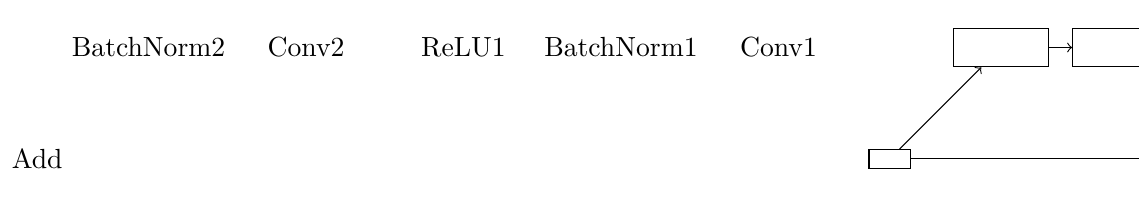
\begin{tikzpicture}[node distance=2cm]
      \node[draw] (input) {קלט};
      \node[draw, above right of=input] (conv1) {Conv1};
      \node[draw, right of=conv1] (bn1) {BatchNorm1};
      \node[draw, right of=bn1] (relu1) {ReLU1};
      \node[draw, right of=relu1] (conv2) {Conv2};
      \node[draw, right of=conv2] (bn2) {BatchNorm2};
      \node[draw, below right of=bn2] (add) {Add};
      \node[draw, right of=add] (relu2) {ReLU2};

      \draw[->] (input) -- (conv1);
      \draw[->] (input) -- (add);
      \draw[->] (conv1) -- (bn1);
      \draw[->] (bn1) -- (relu1);
      \draw[->] (relu1) -- (conv2);
      \draw[->] (conv2) -- (bn2);
      \draw[->] (bn2) -- (add);
      \draw[->] (add) -- (relu2);
    \end{tikzpicture}
  \end{otherlanguage}
  \caption{בלוק שארית, כשמספר הערוצים בקלט ובפלט זהה וגודל הצעד הוא $1$}
  \label{fig:residual-block-same}
\end{figure}

\begin{figure}[htbp]
  \centering
  \begin{otherlanguage}{english}
    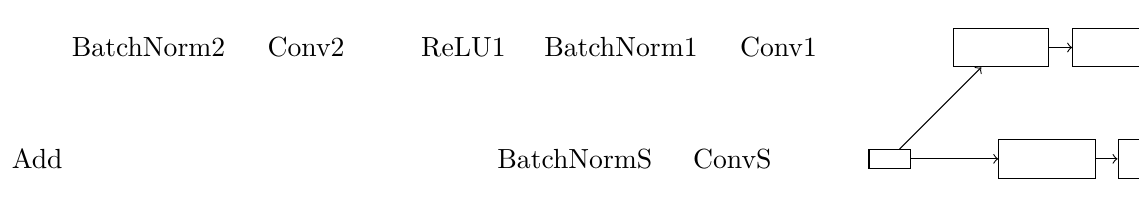
\begin{tikzpicture}[node distance=2cm]
      \node[draw] (input) {קלט};
      \node[draw, above right of=input] (conv1) {Conv1};
      \node[draw, right of=conv1] (bn1) {BatchNorm1};
      \node[draw, right of=bn1] (relu1) {ReLU1};
      \node[draw, right of=relu1] (conv2) {Conv2};
      \node[draw, right of=conv2] (bn2) {BatchNorm2};

      \node[draw, right of=input] (convs) {ConvS};
      \node[draw, right of=convs] (bns) {BatchNormS};

      \node[draw, below right of=bn2] (add) {Add};
      \node[draw, right of=add] (relu2) {ReLU2};

      \draw[->] (input) -- (conv1);
      \draw[->] (conv1) -- (bn1);
      \draw[->] (bn1) -- (relu1);
      \draw[->] (relu1) -- (conv2);
      \draw[->] (conv2) -- (bn2);
      \draw[->] (bn2) -- (add);

      \draw[->] (input) -- (convs);
      \draw[->] (convs) -- (bns);
      \draw[->] (bns) -- (add);

      \draw[->] (add) -- (relu2);
    \end{tikzpicture}
  \end{otherlanguage}
  \caption{בלוק שארית, כשמספר הערוצים בקלט ובפלט שונה או גודל הצעד שונה מ-$1$}
  \label{fig:residual-block-different}
\end{figure}

\begin{table}[htbp]
  \centering
  \begin{tabular}{ccc}
    שם & סוג & פרטים \\\hline
    Conv1 & קונבולוציה & $f$ פילטרים בגודל $k$, גודל צעד $s$, ריפוד \verb|same| \\
    BatchNorm1 & Batch Normalization & \\
    ReLU1 & אקטיבציה & \\
    Conv2 & קונבולוציה & $f$ פילטרים בגודל $k$, גודל צעד $1$, ריפוד \verb|same| \\
    BatchNorm2 & Batch Normalization & \\

    ConvS & קונבולוציה & $f$ פילטרים בגודל $1$, גודל צעד $s$, ריפוד \verb|same| (אם קיימת) \\
    BatchNormS & Batch Normalization & אם קיימת \\

    Add & חיבור & מחברת את הקלטים שלה \\
    ReLU2 & אקטיבציה &
  \end{tabular}
  \caption{פירוט השכבות בבלוק השארית}
  \label{tab:residual-block}
\end{table}

נציין ש\autoref{tab:residual-block} מתארת את השכבות של בלוק שארית
דו-ממדי, אבל השכבות של בלוק שארית חד-ממדי אנלוגיות לחלוטין.

\subsection{מודל חד-ממדי על אודיו גולמי}
\label{sec:architecture-audiocnn}

המודל הזה לא ממיר את הקלט לספקטרוגרמה, ובמקום זאת עובד על האודיו
הגולמי. קלט האודיו הגולמי מאוד ארוך, ולכן הוא מתחיל בשתי שכבות
קונבולוציה יחסית אגרסיביות, במטרה להקטין את ממדי הקלט מהר. לאחר מכן
הוא מעבד את הנתונים באופן יותר עדין.

\begin{center}
  \begin{tabular}{cccc}
    שכבה & סוג & ממדים & פרמטרים \\\hline

    Conv1 & קונבולוציה 1D & $32$ פילטרים באורך $2000$, צעד $26$, ללא ריפוד & $\num{64032}$ \\
    Conv2 & קונבולוציה 1D & $32$ פילטרים באורך $5$ & $\num{5152}$ \\
    BN1 & Batch Normalization & & \\
    Res1 & בלוק שארית 1D & $32$ פילטרים באורך $3$ & $\num{7684}$
  \end{tabular}
\end{center}

\begin{itemize}
\item \textbf{תרשים ארכיטקטורה:} הכינו תרשים שמראה את זרימת הנתונים מקלט לפלט. אפשר TikZ, draw.io, או אפילו ציור ביד שנסרק.
\item \textbf{פירוט שכבות:} טבלה עם סוג השכבה, גודל הקלט, גודל הפלט, מספר פרמטרים
\item \textbf{הסבר בחירות:} \textbf{למה} בחרתם את הארכיטקטורה הזו? מה היתרון?
\item \textbf{מודל בסיס (Backbone):} אם השתמשתם ב-Transfer Learning, מהו מודל הבסיס? אילו שכבות הקפאתם? אילו שיניתם?
\end{itemize}

\section{אימון}
\label{sec:training}

כל המודלים אומנו בעזרת Adam (ראו \autoref{sec:optimization-adam}) עם
שיעור למידה $\num{0.001}$ (או $\num{1e-3}$) למשך $\num{30}$ אפוקים לכל
היותר. בגרסאות קודמות של הפרויקט, עם ארכיטקטורה שונה או אוגמנטציות
שונות, שיעורי למידה גדולים יותר או קטנים יותר עבדו יותר טוב, אבל עבור
הארכיטקטורה הנוכחית (\autoref{sec:architecture}) שיעור למידה הזה הניב
את התוצאות הכי טובות בכל~המודלים.

גודל המקבץ (batch size) נבחר משיקולים פרקטיים, של זיכרון וזמן. מקבצים
מעל $\num{32}$ לקחו יותר מדי זמן באימון, ולכן כל המודלים אומנו בגודל
מקבץ $\num{32}$. כל המודלים השתמשו ב-early stopping, בעזרת המחלקה
המובנית של Keras.

\begin{listing}[htbp]
\inputminted[mathescape]{python}{snippets/Training.py}
\caption{אימון אחד המודלים}
\label{lst:training}
\end{listing}

הפרמטר $m$ עבור הפסד שלישיות (\autoref{sec:triplet-loss}) הוא $0.2$
לכל המודלים.

\begin{itemize}
\item \textbf{היפר-פרמטרים:} Learning Rate, Batch Size, מספר Epochs, Optimizer
\item \textbf{גרפי אימון:} Loss ו-Accuracy (או מדד אחר) לאורך ה-Epochs, עבור Train ו-Validation
\item \textbf{אתגרים ופתרונות:} Overfitting? Underfitting? מודל שלא מתכנס? מה עשיתם?
\item \textbf{ניסויים:} תארו לפחות 2--3 ניסויים שעשיתם (שינוי LR, ארכיטקטורה שונה, אוגמנטציה שונה) --- מה עבד ומה לא?
\item \textbf{זמן אימון:} כמה זמן לקח? על איזו חומרה?
\end{itemize}

\section{השוואת ביצועים}
\label{sec:performance}

\begin{itemize}
\item \textbf{מה ה-Baseline?} נקודת ההשוואה שלכם. למשל:
  \begin{itemize}
  \item ניחוש אקראי (Random)
  \item מודל פשוט (למשל Logistic Regression על פיצ'רים ידניים)
  \item מודל מוכן מהמדף (DeepFace, Resemblyzer)
  \item תוצאות שדווחו במאמר / ב-Kaggle
  \end{itemize}
\item \textbf{טבלת השוואה:} מודל, מדד, תוצאה --- מינימום 3 שורות
\item \textbf{ניתוח:} למה המודל שלכם טוב/פחות טוב? מה המסקנה?
\end{itemize}

\section{תוצאות והדגמות}
\label{sec:results}

\begin{itemize}
\item \textbf{תוצאות כמותיות:} טבלאות מדדים (Accuracy, mAP, F1, RMSE --- לפי סוג הפרויקט)
\item \textbf{דוגמאות הצלחה:} 4--6 דוגמאות שבהן המודל צדק --- הראו קלט ופלט
\item \textbf{דוגמאות כישלון:} 2--3 דוגמאות שבהן המודל טעה --- \textbf{למה} הוא טעה?
\item \textbf{Confusion Matrix:} אם רלוונטי --- מה הדפוסים? איפה המודל מתבלבל?
\item \textbf{צילומי מסך של ההדגמה:} ממשק Gradio / Streamlit / אפליקציה
\item \textbf{קישור לסרטון הדגמה}
\end{itemize}

\section{דיון}
\label{sec:discussion}

\begin{itemize}
\item \textbf{ניתוח תוצאות:} מה עובד? מה לא? מה מפתיע?
\item \textbf{מגבלות:} באילו מצבים המודל נכשל? מה ה-edge cases?
\item \textbf{השוואה למצב הקיים:} איפה הפרויקט שלכם עומד ביחס ל-state of the art?
\item \textbf{הצעות לשיפור:} אם היו לכם עוד 3 חודשים, מה הייתם משפרים?
\item \textbf{שיקולים אתיים:} (אם רלוונטי) פרטיות, הטיה, שימוש לרעה
\end{itemize}

\section{רפלקציה}
\label{sec:reflection}

\begin{itemize}
\item \textbf{תהליך הלמידה:} מה למדתם שלא ידעתם קודם?
\item \textbf{הרגע הקשה ביותר:} מה היה האתגר הכי גדול? איך התמודדתם?
\item \textbf{הרגע המרגש ביותר:} מתי הרגשתם ש"זה עובד!"?
\item \textbf{ניהול זמן:} האם הצלחתם לעמוד בלוח הזמנים? מה הייתם עושים אחרת?
\item \textbf{מה הייתם עושים אחרת?} אם הייתם מתחילים מחדש, מה הייתם משנים?
\item \textbf{איפה אתם רוצים להמשיך?} האם הפרויקט עורר בכם עניין להמשיך לתחום?
\end{itemize}

\appendix

\section{קטעי קוד נבחרים}
\label{sec:code}

\subsection{מערך הנתונים}
\label{sec:code-dataset}

\subsubsection{קריאת נתוני השמע (חלק מהפונקציות הושמטו)}
\label{sec:code-triple-audio-dataset}

\inputminted{python}{snippets/TripleAudioDataset.py}

\subsubsection{בניית ספקטרוגרמות Mel (חלק מהפונקציות הושמטו)}
\label{sec:code-mel-spectrogram}

\inputminted[texcomments]{python}{snippets/LogMelSpectrogram.py}

\subsection{מודלים}
\label{sec:code-models}

\section{סיכומי מודלים}
\label{sec:summaries}

\section{גרפים וטבלאות}
\label{sec:graphs}

% \begin{otherlanguage}{english}
%   \printbibliography[heading=bibintoc,title={מקורות}]
% \end{otherlanguage}

\cleardoublepage

\phantomsection
\addcontentsline{toc}{section}{\listfigurename}
\listoffigures

\phantomsection
\addcontentsline{toc}{section}{\listtablename}
\listoftables

\phantomsection
\addcontentsline{toc}{section}{\listlistingname}
\listoflistings

\end{document}
